\documentclass[11pt]{article}

\usepackage[margin=1in]{geometry}
\usepackage{amsmath,amssymb}
\usepackage{graphicx}
\usepackage{booktabs}
\usepackage{array}
\usepackage{hyperref}
\usepackage{caption}
\usepackage{subcaption}
\usepackage{enumitem}
\usepackage{xcolor}
\usepackage{microtype}

\hypersetup{
    colorlinks=true,
    linkcolor=blue!55!black,
    citecolor=blue!55!black,
    urlcolor=blue!55!black
}

\title{Regulatory State Modulation Reduces Post-Error Burden in Stochastic Tool-Using Agents}
\author{Veronique Ziegler\\Critical Attention Systems}
\date{\today}

\begin{document}
\maketitle

\begin{abstract}
Tool-using agents fail not only by choosing wrong actions, but also by persisting after failure. A failed tool call creates a local disturbance: an assumption about the task environment has been contradicted. The agent must then decide whether to repeat the failed action, inspect the environment, make a new guess, or stop and answer. This paper studies post-error burden as a measurable control problem in stochastic tool-using agents. We evaluate a Critical Attention Systems (CAS) Agent Governor that modulates action-selection probabilities according to regulatory state rather than directly solving the task. The governor does not know the correct file path and does not prescribe task-specific recovery steps. It changes broad action tendencies after disturbance: repeated failed actions are down-weighted, uncertainty-reducing inspections are favored, and final answering is favored only after evidence has been recovered. The experiment uses eight file-recovery tasks, five stochastic agent types, two conditions, and 10,000 random seeds per task-condition pair, for 800,000 total runs. CAS regulation reduces post-error burden for exploratory, clinging, persistent, and noisy agents, with the strongest effect for persistent agents: success increases from 0.739 to 0.973 and mean post-error burden falls from 8.574 to 3.007. Repeated failed actions are suppressed to zero in the governed condition across all five agent types. The impulsive agent shows a boundary condition: governance slightly reduces success and increases burden. These results support a narrow claim: regulatory state modulation is useful when the dominant failure mode is perseverative or noisy recovery, but it is not a general agent-intelligence improvement and not a substitute for task competence.
\end{abstract}

\section{Introduction}

Tool-using agents fail not only by choosing wrong actions, but by persisting after failure. A wrong file path, an empty directory, or a failed tool call does not necessarily make a task impossible. It changes the control situation. The agent's current assumption has been contradicted, and the next useful behavior is usually not blind repetition. The agent should reduce uncertainty, use recovered evidence, and stop when the relevant evidence is sufficient.

This paper studies that recovery process as a measurable control problem. The central quantity is \emph{post-error burden}: the amount of tool use required after the first failed action. A high post-error burden indicates that the agent continues to spend control effort after disturbance. This may happen because the agent repeats a failed action, guesses without new evidence, searches inefficiently, or continues tool use after the answer is already available.

The aim is not to test broad language understanding or benchmark a commercial language model. Instead, the aim is to isolate a regulatory mechanism in a reproducible stochastic environment. The question is whether a generic regulatory signal can reduce repeated failed actions and post-error burden without giving the agent the solution path.

We evaluate a CAS Agent Governor in a file-recovery domain. The governor observes the history of tool use and assigns a regulatory state: normal, disturbed, recovering, stuck, or released. These states do not encode the task answer. They modulate broad action classes. For example, after a failed action, retrying the same failed action becomes less likely and uncertainty-reducing inspection becomes more likely. After useful evidence is recovered, repeated search becomes less likely and final answering becomes more likely.

The contribution is a controlled stochastic study of regulatory state modulation in tool-using agents. The results show strong benefits for agents whose dominant failure mode is perseveration or noisy recovery, and a clear boundary condition for impulsive agents. This qualification is important: the result is not that regulation always improves every agent. The result is that regulation is useful when the agent's failure mode is post-error persistence.

\section{Background}

\subsection{CAS and IRAM-$\Omega$-Q motivation}

Critical Attention Systems (CAS) and the IRAM-$\Omega$-Q framework treat regulation as a central feature of artificial agency. The relevant question is not only whether an agent can select an action, but how it responds when its current action policy encounters uncertainty, disturbance, or contradiction. In this view, failures are not merely local errors. They create a regulatory condition: the agent must adjust control effort, reduce uncertainty, avoid looping, and release control once sufficient evidence has been recovered.

The present study applies that idea in a deliberately narrow setting. The agent is not modeled as conscious, and no claim is made about general intelligence. The experiment only asks whether regulatory state modulation can reduce measurable post-error burden in stochastic tool use. This keeps the application close to observable behavior: tool calls, failed actions, repeated failures, and successful recovery.

\subsection{Regulation as state-dependent modulation}

The CAS Agent Governor is not a planner. It does not choose the correct file, does not know the directory layout in advance, and does not insert task-specific hints. Its role is to evaluate the interaction history and modulate action tendencies.

Let $h_t$ denote the history of actions and results up to step $t$. The governor maps this history to a regulatory signal
\begin{equation}
    r_t = (s_t, b_t, m_t),
\end{equation}
where $s_t$ is the regulatory state, $b_t$ is a burden score, and $m_t$ is a short diagnostic message. The regulatory state changes how strongly the agent favors broad classes of action. It does not directly specify the task solution.

For a candidate action $a$ and history $h_t$, the stochastic agent samples from a policy
\begin{equation}
    P(a \mid h_t, s_t) = \frac{w(a; h_t, s_t)}{\sum_{a' \in \mathcal{A}(h_t)} w(a'; h_t, s_t)},
\end{equation}
where $\mathcal{A}(h_t)$ is the set of candidate actions available at the current step. In the ungoverned condition, weights are determined by the baseline stochastic policy. In the governed condition, the same baseline weights are modulated by the CAS state.

\subsection{Disturbance, recovery, and burden}

A failed tool call is treated as a disturbance. It indicates that a current assumption has failed. Recovery begins when the agent obtains useful evidence after disturbance, such as a successful directory listing or a successful read of a relevant file. Burden is the cost of getting from disturbance to recovery and final answer.

The important distinction is between task solving and regulation. A task-solving system may know where to look. A regulatory system does not need to know where to look. It needs to reduce unproductive persistence after failure and favor information-gathering actions when the current assumption has broken down.

\section{Stochastic Tool-Use Model}

\subsection{Agent types}

Five stochastic agent types are used. They differ only in baseline action-selection weights.

\begin{center}
\begin{tabular}{p{0.22\linewidth} p{0.68\linewidth}}
\toprule
\textbf{Agent type} & \textbf{Baseline tendency} \\
\midrule
Exploratory & Low retry tendency and relatively high inspection tendency. \\
Clinging & Medium-to-high tendency to repeat a failed action. \\
Persistent & Strong tendency to repeat a failed action after disturbance. \\
Impulsive & Elevated tendency to answer before sufficient evidence has been recovered. \\
Noisy & Elevated tendency to make unsupported guesses or noisy exploratory moves. \\
\bottomrule
\end{tabular}
\end{center}

These agent types are not intended as full cognitive models. They are controlled failure-mode models. Each type represents a different way a tool-using agent can fail after an initial disturbance.

\subsection{Tool semantics}

The simulated agent interacts with a small file workspace through two tool actions: \texttt{READ\_FILE} and \texttt{LIST\_DIRECTORY}. These tools are deliberately simple. They are not search engines and they do not perform semantic retrieval.

A \texttt{READ\_FILE} action takes a single relative file path as its target. The action succeeds only if that exact path exists in the workspace and refers to a file. If the path is absent, misspelled, points to a directory, or is otherwise invalid, the action fails and returns an error. Thus, \texttt{READ\_FILE} tests a specific hypothesis about where the needed information is located. It does not inspect neighboring files, list directories, or suggest alternatives.

A \texttt{LIST\_DIRECTORY} action takes a single relative directory path as its target. The action succeeds only if that exact path exists and refers to a directory. On success, it returns the immediate entries in that directory. It does not recursively search subdirectories. In the model, \texttt{LIST\_DIRECTORY} is the main uncertainty-reducing action available after a failed file read.

This distinction is central to the experiment. A failed \texttt{READ\_FILE} action represents a failed commitment to a specific assumption. Repeating the same failed read without new evidence is counted as a repeated failed action. By contrast, using \texttt{LIST\_DIRECTORY} after a failed read represents a shift from commitment to inspection: the agent reduces uncertainty about the workspace before attempting another file read.

For example, suppose the task prompt suggests the path \texttt{examples/trial\_config.json}, but the actual file is located at \texttt{configs/trial\_config\_demo.json}. If the agent calls \texttt{READ\_FILE} on \texttt{examples/trial\_config.json}, the tool returns \texttt{FILE\_NOT\_FOUND}. A perseverative agent may call the same failed read again, increasing post-error burden. A recovering agent may instead call \texttt{LIST\_DIRECTORY} on a candidate directory or on the workspace root, observe the available directories, and then issue a new \texttt{READ\_FILE} only after obtaining evidence for a candidate path.

\subsection{Tool actions and failure modes}

The environment exposes two file tools and one final-answer action:

\begin{enumerate}[leftmargin=1.5em]
    \item \texttt{READ\_FILE(target)} reads a file at a relative path.
    \item \texttt{LIST\_DIRECTORY(target)} lists a directory at a relative path.
    \item \texttt{FINAL\_ANSWER} ends the run with an answer.
\end{enumerate}

The stochastic policy includes broad action classes:

\begin{itemize}[leftmargin=1.5em]
    \item retry the last failed action;
    \item inspect the current or candidate environment;
    \item read a candidate file;
    \item make a random guess;
    \item answer prematurely.
\end{itemize}

The ungoverned agent samples from these action classes according to its baseline weights. The governed agent uses the same baseline policy, but the CAS state changes the weights after disturbance.

\subsection{CAS states}

The governor uses five regulatory states.

\begin{center}
\begin{tabular}{p{0.20\linewidth} p{0.70\linewidth}}
\toprule
\textbf{State} & \textbf{Operational meaning} \\
\midrule
NORMAL & No recent disturbance has been detected. The agent proceeds with its baseline policy. \\
DISTURBED & A recent action failed. Blind repetition is down-weighted and uncertainty reduction is favored. \\
RECOVERING & Useful information has been obtained after disturbance. The agent should continue from recovered evidence. \\
STUCK & Repeated failure or looping is occurring. The failed strategy is strongly suppressed. \\
RELEASED & Sufficient task-relevant evidence has been recovered. Final answering is favored. \\
\bottomrule
\end{tabular}
\end{center}

These states implement regulation as state-dependent modulation, not direct task solving. The governor can alter the probability of retrying, inspecting, reading, or answering, but it does not provide the correct filename or directory.

\section{Experimental Design}

The experiment uses eight file-recovery tasks. Each task contains a recoverable target file but presents the agent with an initial misleading or incomplete path assumption. The task types include wrong filenames, wrong folders, wrong extensions, empty expected directories, competing similar filenames, stale filenames, nested directories, and latest-summary recovery.

Each task was constructed so that the prompt contained an initially plausible but unreliable path cue. The correct file existed in the workspace, but recovering it often required moving from a failed \texttt{READ\_FILE} attempt to one or more \texttt{LIST\_DIRECTORY} inspections. This design makes post-error behavior observable: the experiment measures whether an agent repeats a failed commitment, makes unsupported guesses, or shifts toward uncertainty reduction.

Each task is run with five stochastic agent types under two conditions:

\begin{itemize}[leftmargin=1.5em]
    \item \textbf{Ungoverned}: the agent samples actions from its baseline stochastic policy.
    \item \textbf{Governed}: the agent samples actions from the same baseline policy after CAS state modulation.
\end{itemize}

The publication configuration is:

\begin{center}
\begin{tabular}{ll}
\toprule
\textbf{Parameter} & \textbf{Value} \\
\midrule
Maximum steps per run & 16 \\
Seeds per task-condition pair & 10,000 \\
Tasks & 8 \\
Agent types & 5 \\
Conditions & Ungoverned, governed \\
Total runs & $8 \times 5 \times 2 \times 10{,}000 = 800{,}000$ \\
\bottomrule
\end{tabular}
\end{center}

In code, the publication settings are:

\begin{verbatim}
private static final int MAX_STEPS = 16;
private static final int SEEDS_PER_CONDITION = 10000;
\end{verbatim}

The random seeds are repeated across conditions so that governed and ungoverned runs are comparable at the level of agent type and task family. Each aggregate result reported below combines 80,000 runs: eight tasks times 10,000 random seeds for one agent type and condition.

\section{Metrics}

The analysis uses the following metrics.

\begin{itemize}[leftmargin=1.5em]
    \item \textbf{Success rate}: fraction of runs in which the expected target file is recovered and the final answer is produced.
    \item \textbf{Total tool calls}: mean number of tool calls per run.
    \item \textbf{Failed tool calls}: mean number of failed tool calls per run.
    \item \textbf{Repeated failed actions}: mean number of times the agent repeats an action that already failed.
    \item \textbf{Post-error tool burden}: mean number of tool calls after the first failed action.
    \item \textbf{Regulatory signals}: mean number of CAS state signals emitted during governed runs.
    \item \textbf{Soft warnings and hard blocks}: mean number of governor interventions.
\end{itemize}

A repeated failed action is counted when the agent issues the same tool action with the same target after that action has already failed, without an intervening successful action that provides new information. In practice, the most common repeated failure is a repeated \texttt{READ\_FILE} call on a path that has already returned \texttt{FILE\_NOT\_FOUND}.

Post-error burden is the primary outcome. It measures the control cost of recovery after disturbance. Repeated failed actions are a more specific measure of perseveration. Success rate measures whether burden reduction is achieved without destroying task completion.

\section{Results}

\subsection{Aggregate outcomes}

Table~\ref{tab:main-results} summarizes the aggregate outcomes. CAS regulation reduces post-error burden for exploratory, clinging, persistent, and noisy agents. The largest reduction occurs for persistent agents. The impulsive agent shows a boundary condition: governance slightly reduces success and increases burden.

\begin{table}[htbp]
\centering
\caption{Aggregate stochastic-policy results. Each row aggregates 80,000 runs. Burden reduction is computed as $(B_{ungoverned}-B_{governed})/B_{ungoverned}$.}
\label{tab:main-results}
\begin{tabular}{lrrrrr}
\toprule
Agent type & Success ungov. & Success gov. & Burden ungov. & Burden gov. & Burden reduction \\
\midrule
Exploratory & 0.979 & 0.980 & 2.014 & 1.011 & 49.8\% \\
Clinging & 0.909 & 0.984 & 5.707 & 2.520 & 55.8\% \\
Persistent & 0.739 & 0.973 & 8.574 & 3.007 & 64.9\% \\
Impulsive & 0.998 & 0.972 & 1.493 & 1.708 & -14.4\% \\
Noisy & 0.893 & 0.938 & 5.611 & 3.035 & 45.9\% \\
\bottomrule
\end{tabular}
\end{table}

\subsection{Post-error burden reduction}

Figure~\ref{fig:burden} shows the primary result. CAS regulation reduces post-error burden for four of the five stochastic agent types. The strongest effect occurs for persistent agents, where mean post-error burden falls from 8.574 to 3.007. Clinging and noisy agents also show large reductions.

\begin{figure}[htbp]
\centering
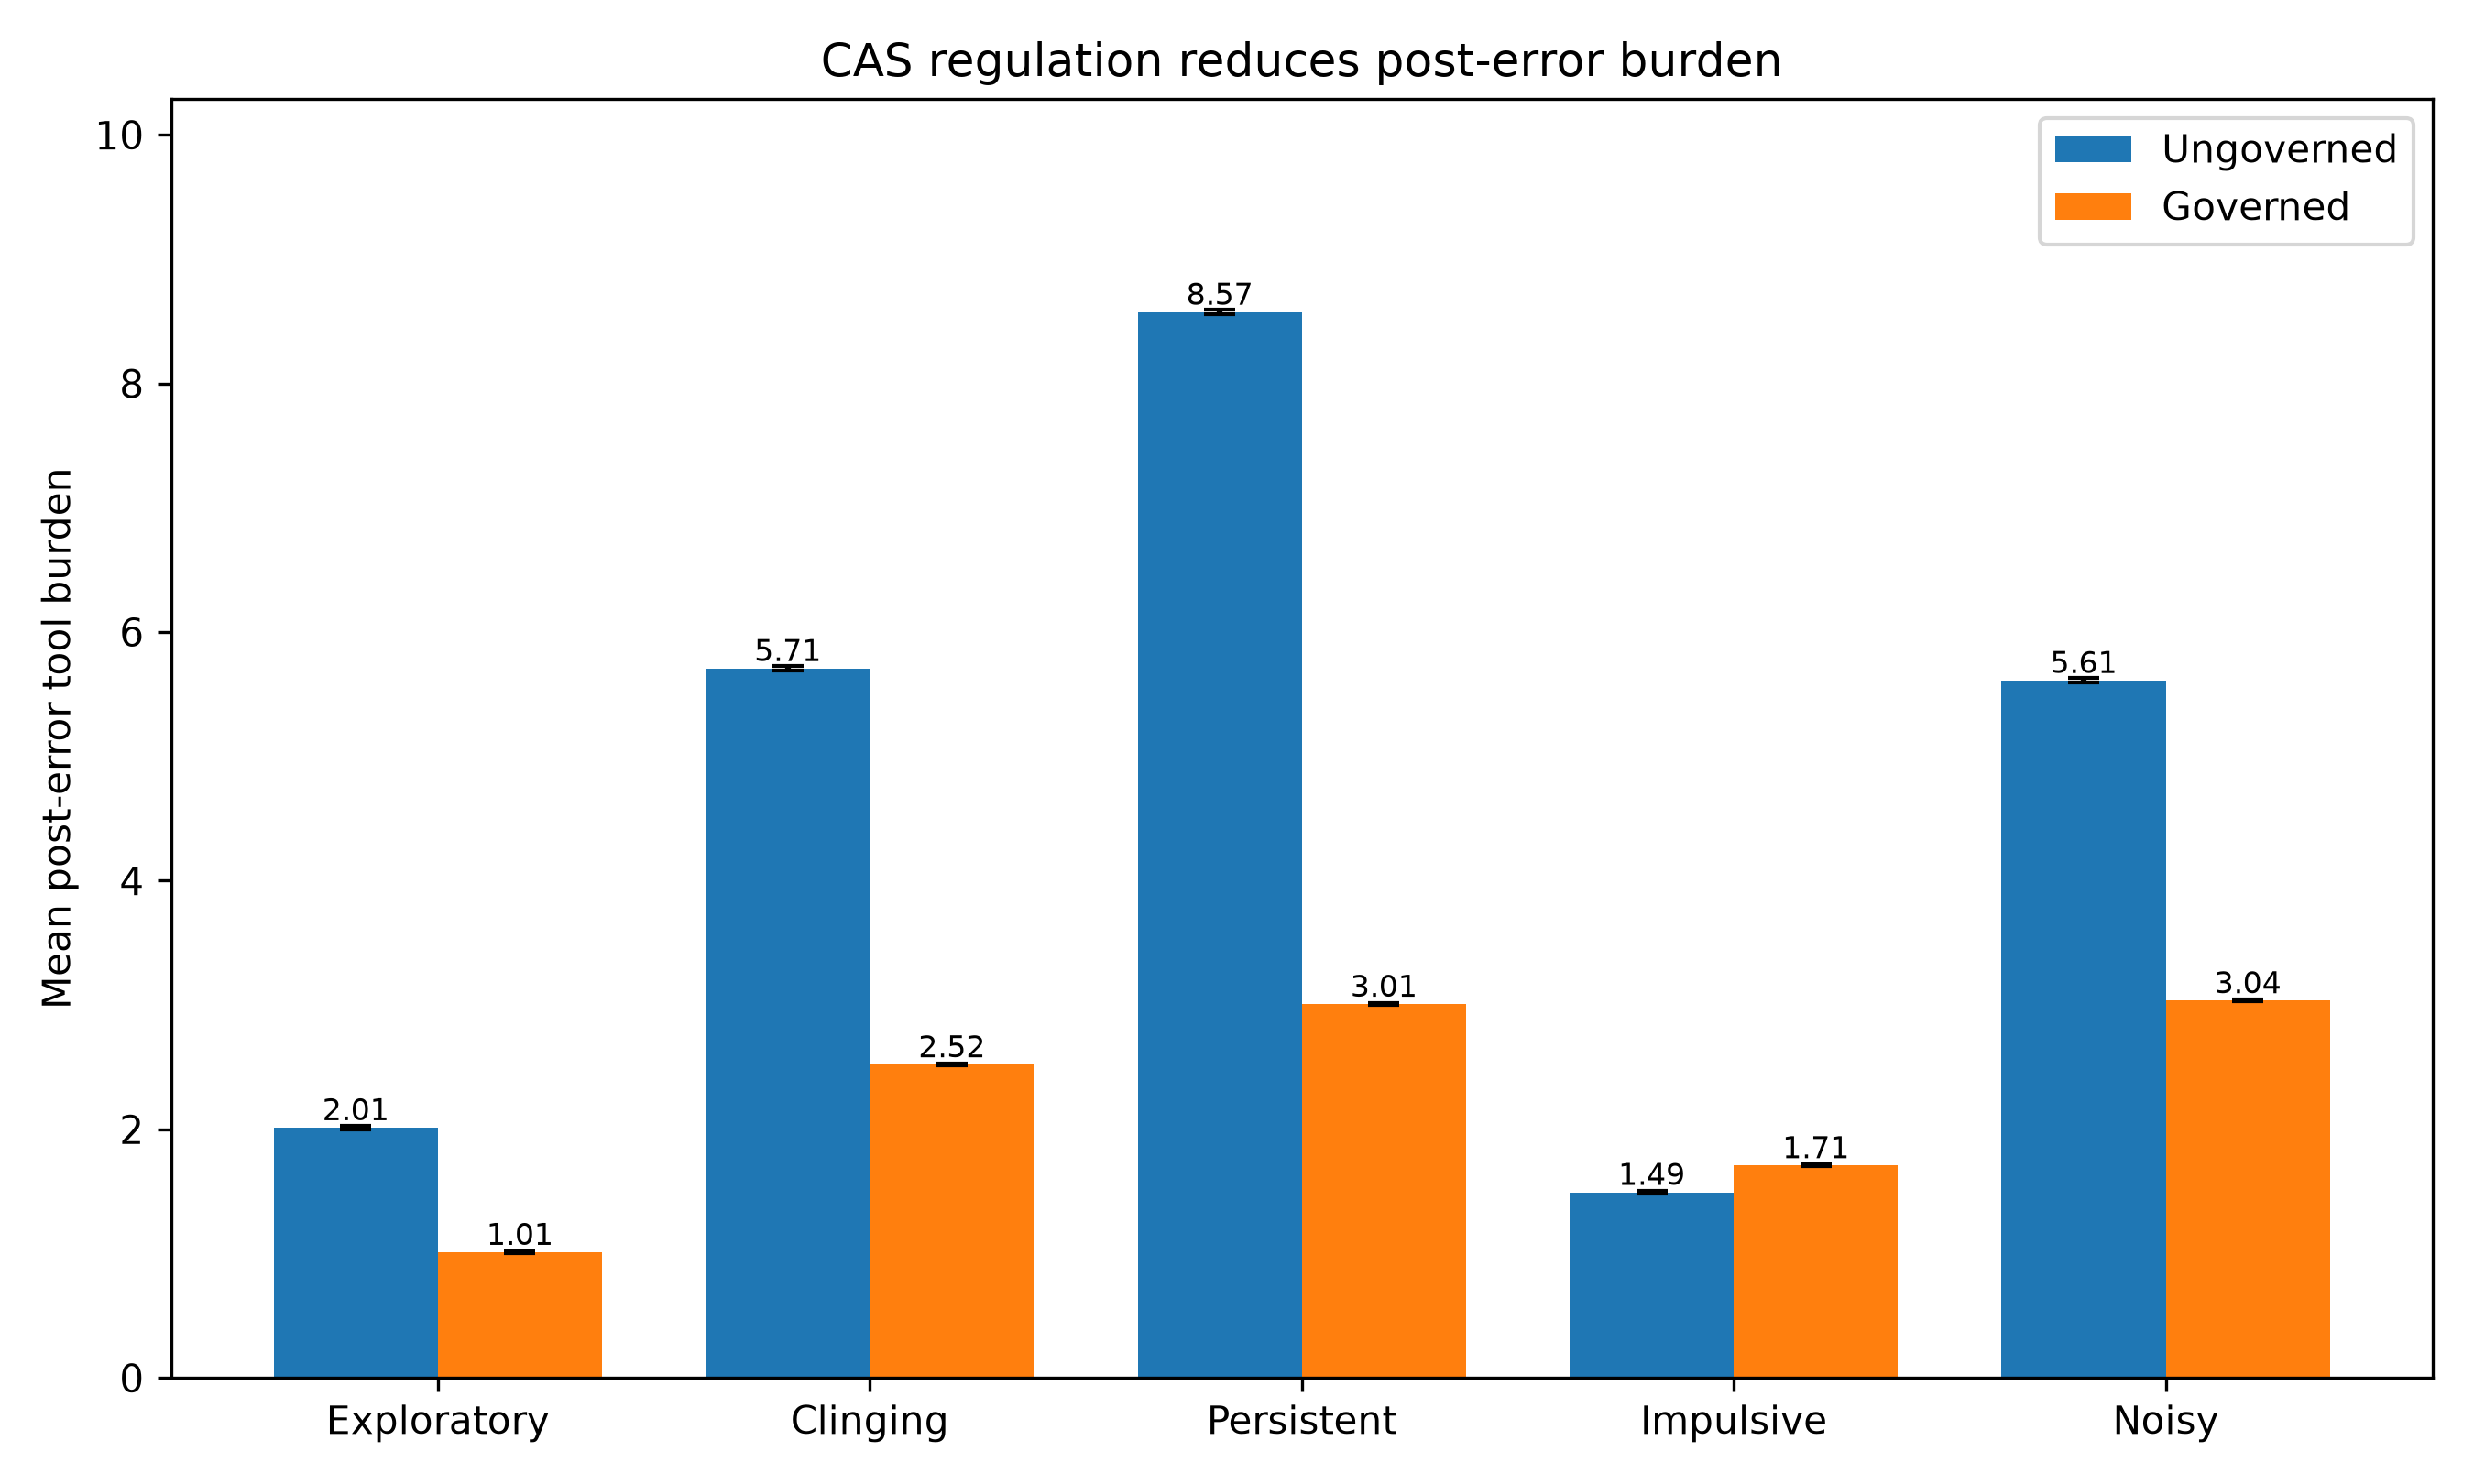
\includegraphics[width=0.92\linewidth]{figures/post_error_burden_by_agent_type.png}
\caption{Mean post-error tool burden by agent failure mode. Error bars show standard error. CAS regulation reduces burden for exploratory, clinging, persistent, and noisy agents, while increasing burden for the impulsive agent.}
\label{fig:burden}
\end{figure}

\subsection{Repeated failed actions suppressed}

Figure~\ref{fig:repeated} shows the clearest regulatory effect. In the governed condition, repeated failed actions are suppressed to zero across all five agent types. This is the direct behavioral signature of the governor's post-error modulation: after disturbance, blind repetition of a failed action is suppressed.

\begin{figure}[htbp]
\centering
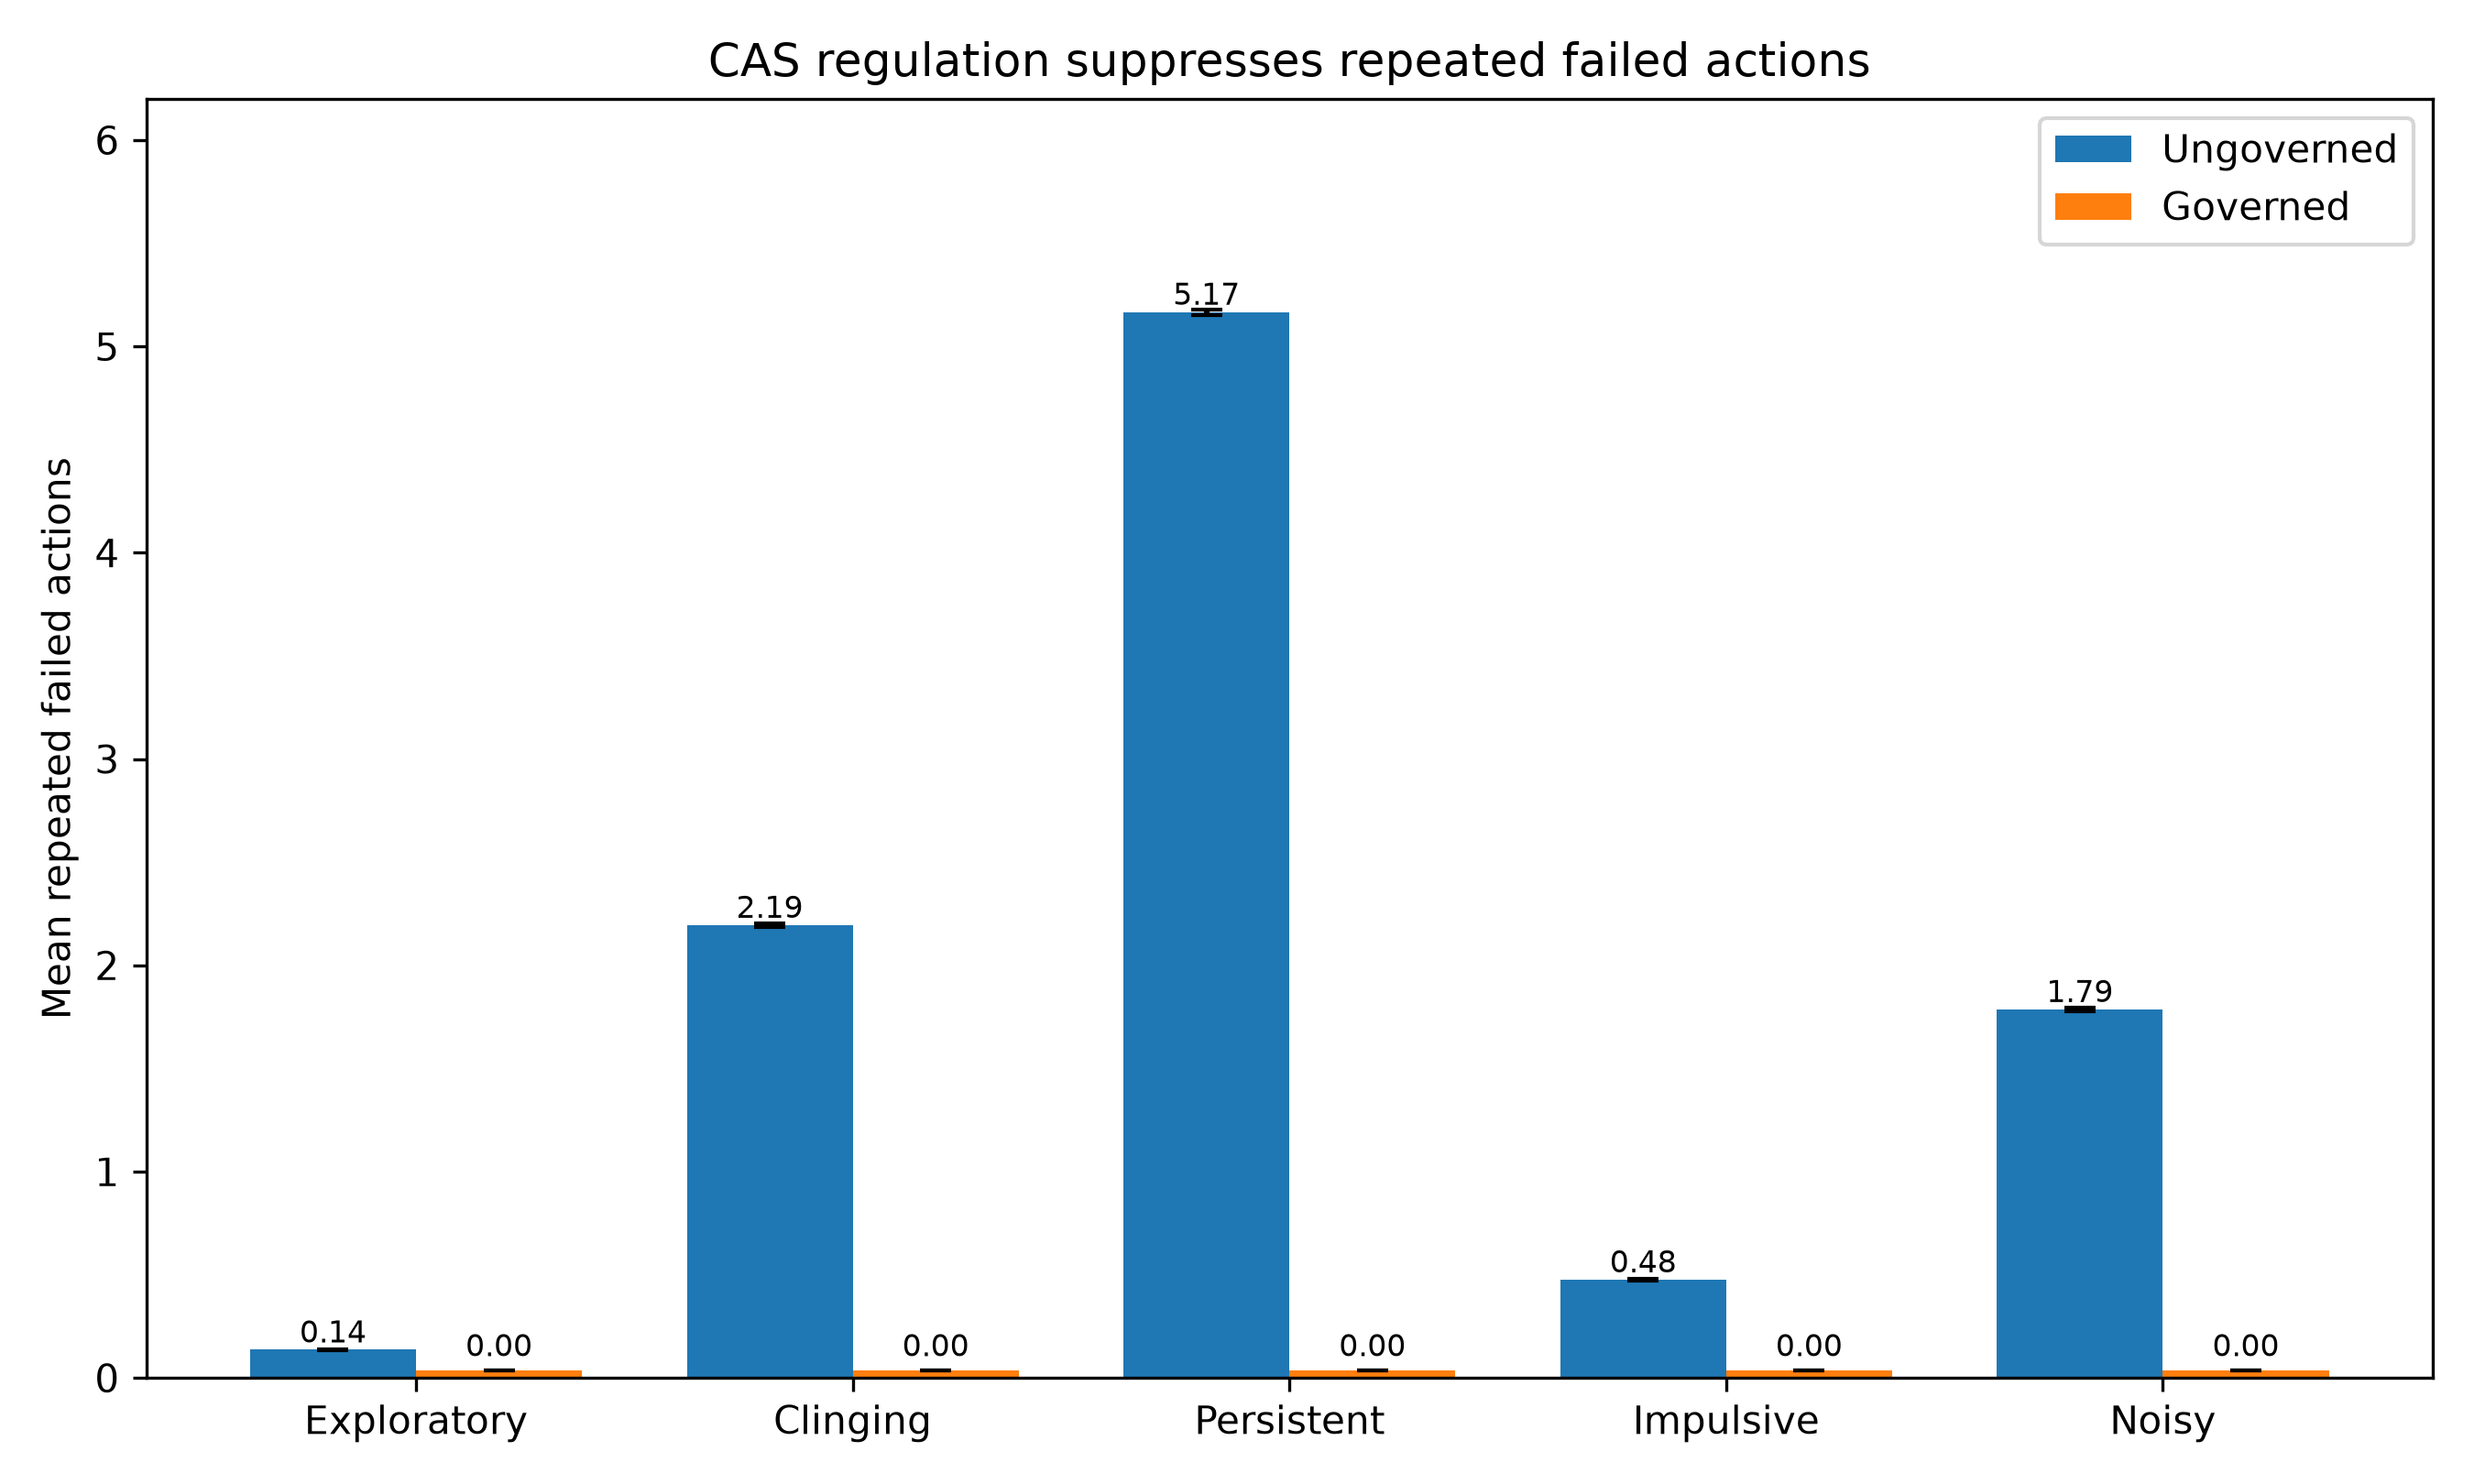
\includegraphics[width=0.92\linewidth]{figures/repeated_failed_actions_by_agent_type.png}
\caption{Mean repeated failed actions by agent failure mode. The governed condition is plotted side-by-side with the ungoverned condition. CAS regulation suppresses repeated failed actions to zero across all five tested agent types.}
\label{fig:repeated}
\end{figure}

\subsection{Success improved for clinging, persistent, and noisy agents}

Figure~\ref{fig:success} shows that success improves for clinging, persistent, and noisy agents. The persistent agent shows the largest success improvement, rising from 0.739 to 0.973. This matters because burden reduction alone would be weak if it came from premature stopping. The persistent and clinging results show reduced burden together with improved success.

\begin{figure}[htbp]
\centering
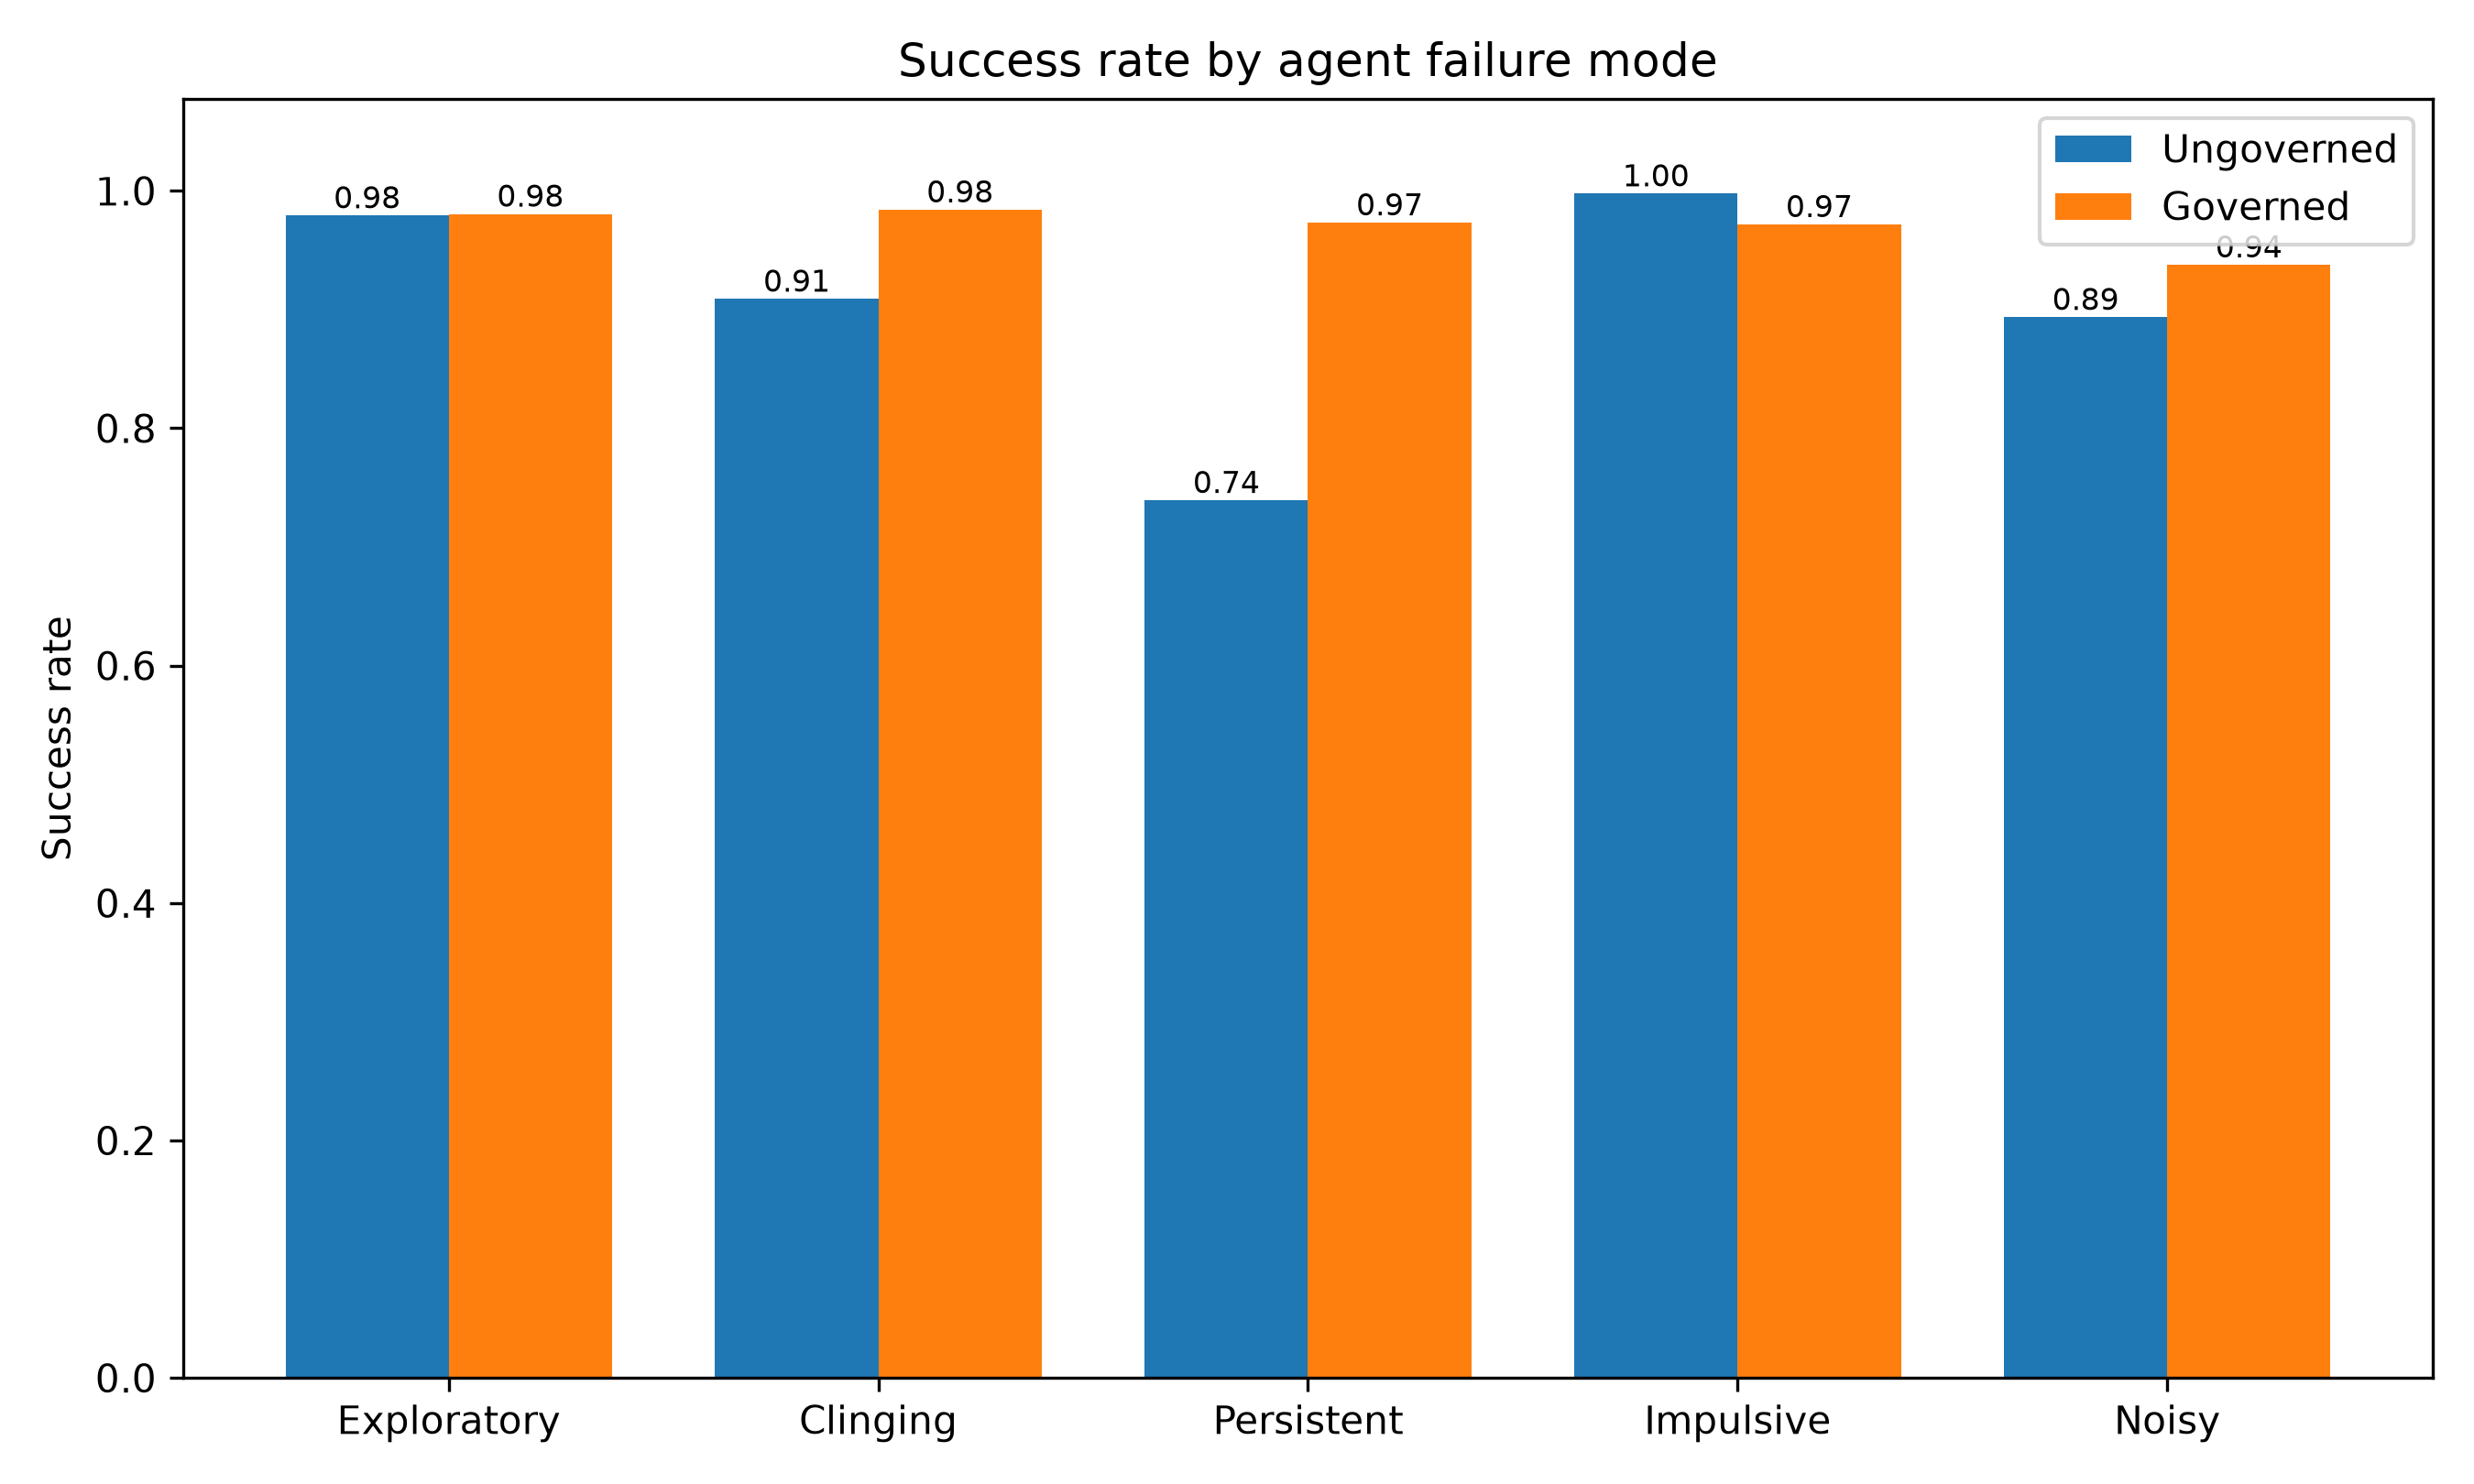
\includegraphics[width=0.92\linewidth]{figures/success_rate_by_agent_type.png}
\caption{Success rate by agent failure mode. CAS regulation improves success for clinging, persistent, and noisy agents, remains nearly unchanged for exploratory agents, and produces a small success penalty for impulsive agents.}
\label{fig:success}
\end{figure}

\subsection{Impulsive boundary condition}

The impulsive agent provides an important boundary condition. Its ungoverned success rate is already high, and its baseline behavior is not dominated by repeated failed actions. Under governance, its success rate decreases from 0.998 to 0.972 and its post-error burden increases from 1.493 to 1.708. This result should not be hidden. It shows that regulation is not universally beneficial. It helps when the failure mode is post-error persistence, but it can impose cost when the baseline policy is already fast and the dominant failure is not perseveration.

Figure~\ref{fig:reduction} expresses the burden effect as a percentage. The persistent agent has the largest reduction at 64.9\%, followed by clinging at 55.8\%, exploratory at 49.8\%, and noisy at 45.9\%. The impulsive agent shows a negative burden reduction of -14.4\%.

\begin{figure}[htbp]
\centering
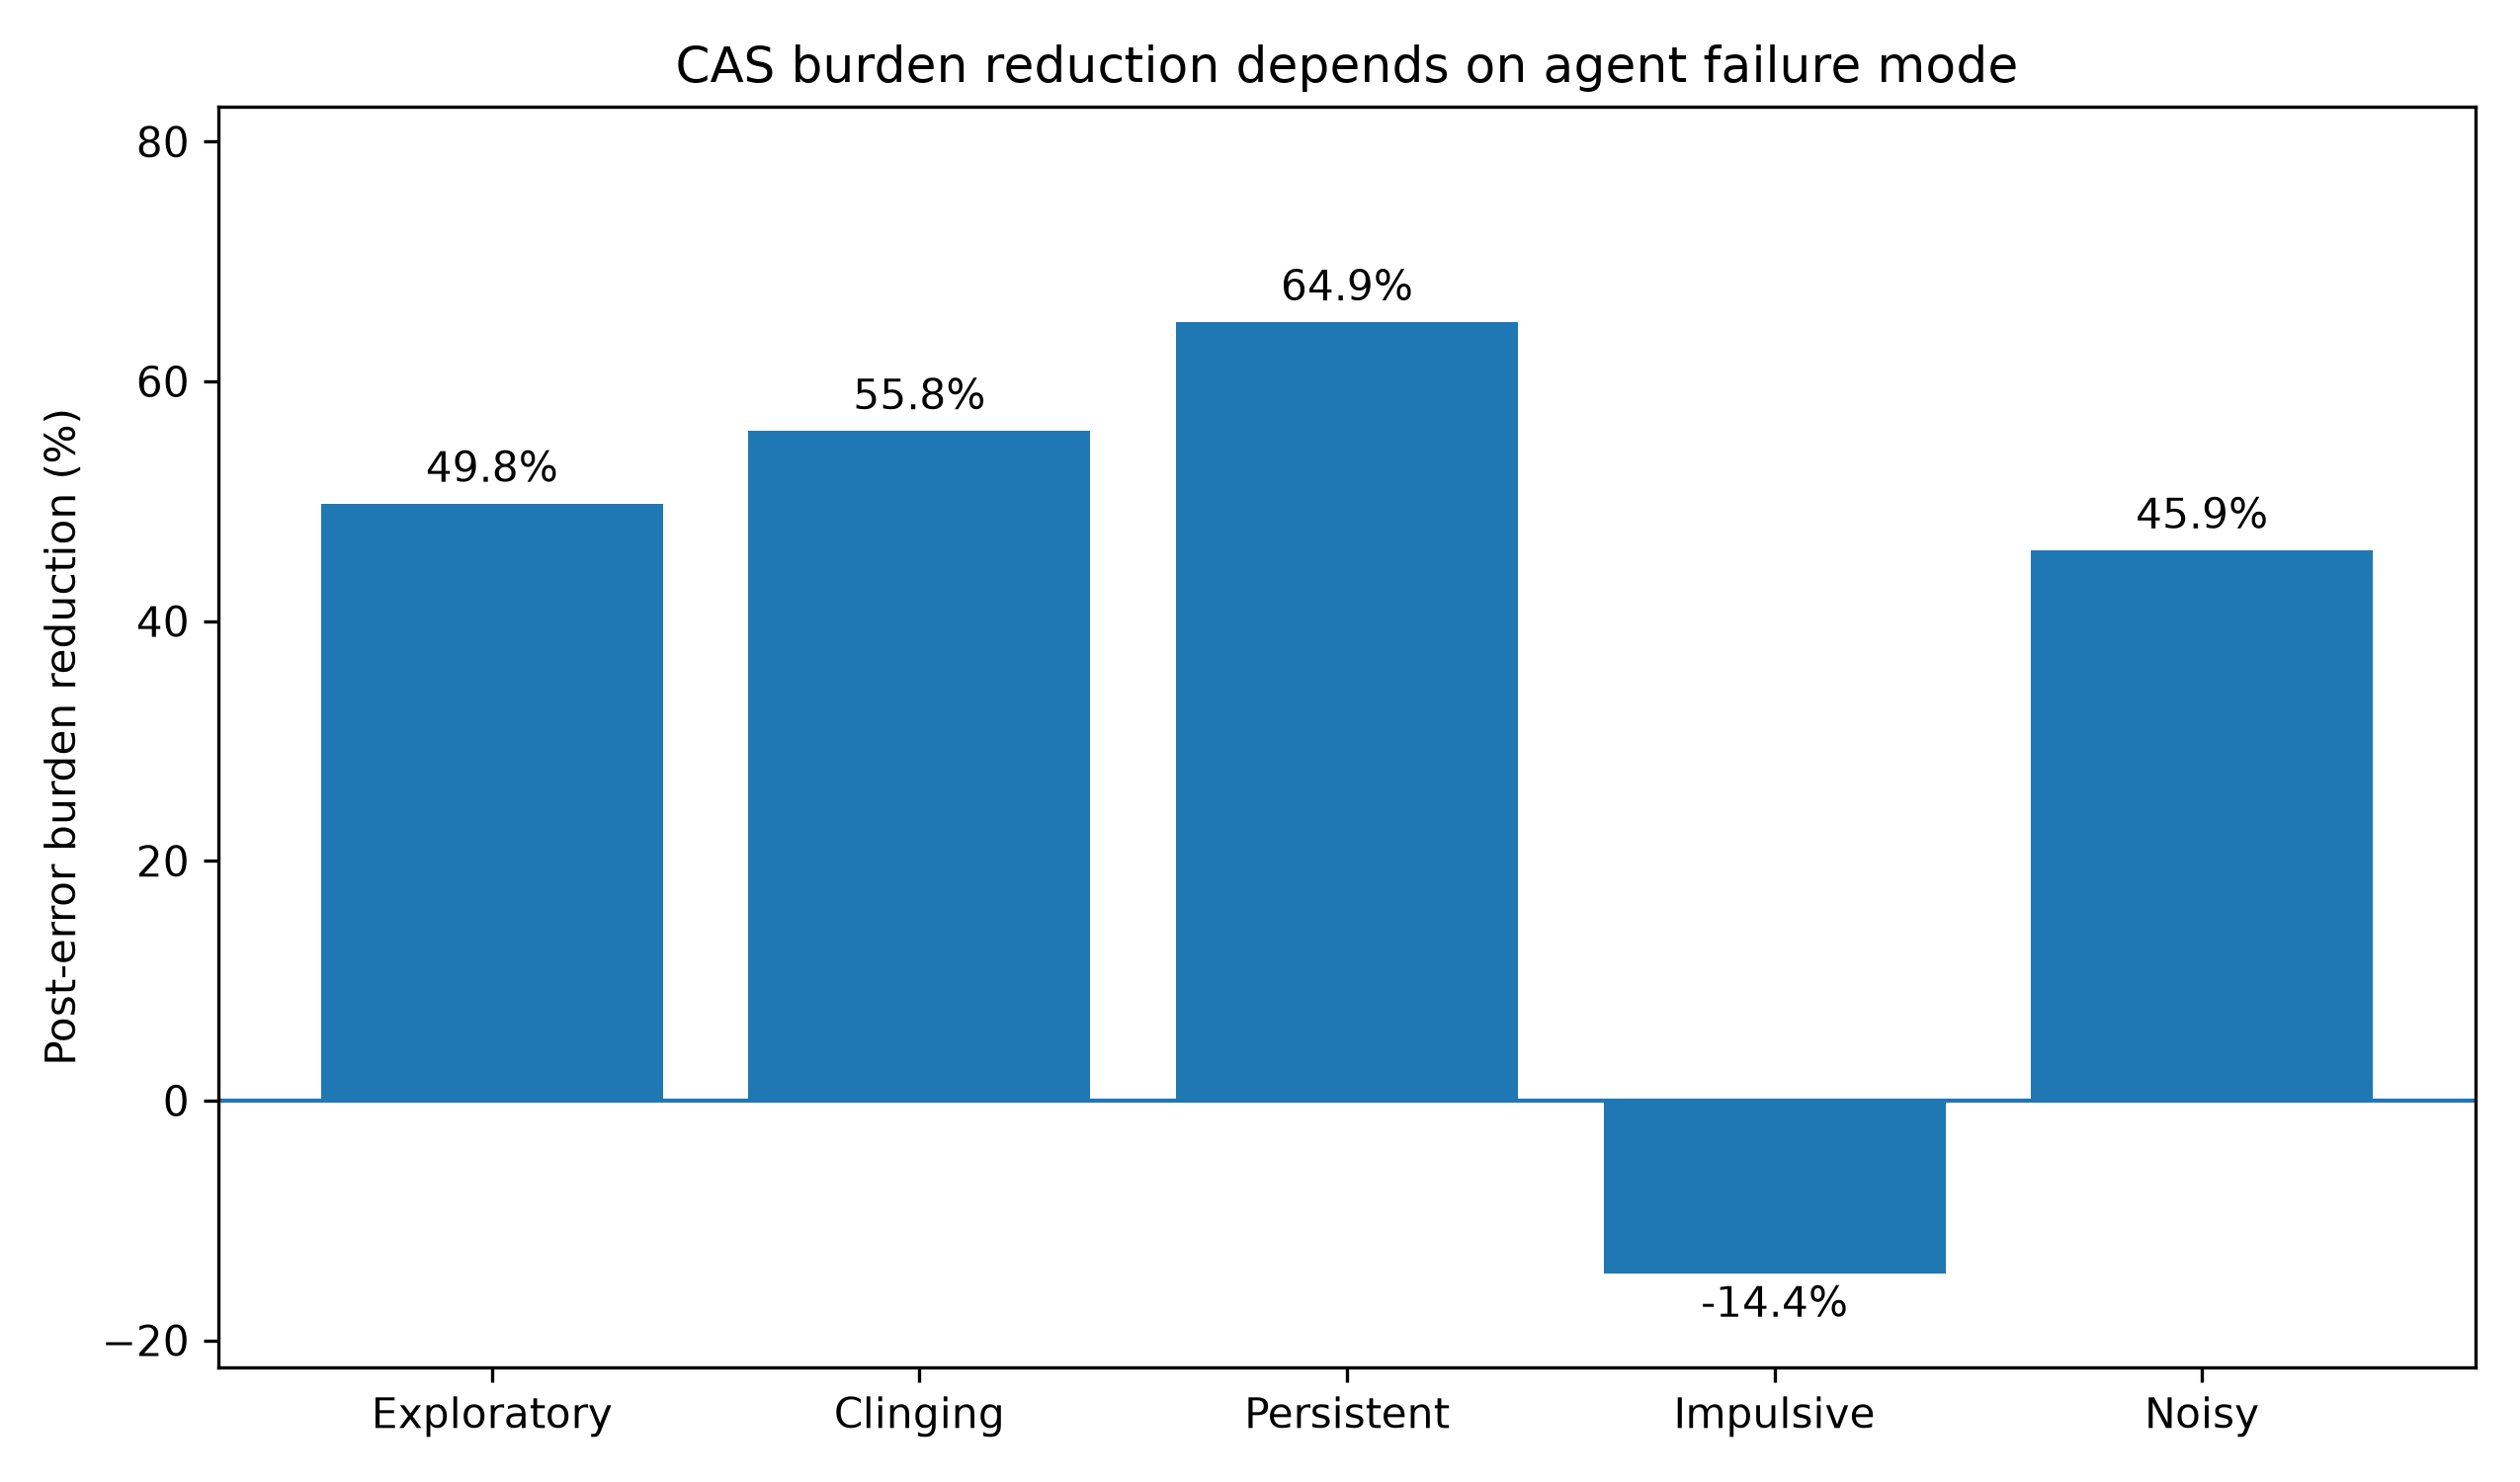
\includegraphics[width=0.92\linewidth]{figures/post_error_burden_reduction_percent.png}
\caption{Post-error burden reduction by agent failure mode. Positive values indicate reduced burden under CAS regulation. The negative impulsive result shows that regulatory modulation can add cost when the baseline agent is not primarily perseverative.}
\label{fig:reduction}
\end{figure}

\subsection{Success-burden tradeoff}

Figure~\ref{fig:tradeoff} summarizes the success-burden relationship as a change plot. The horizontal axis shows post-error burden reduction under governance. The vertical axis shows success-rate change under governance. Clinging, persistent, and noisy agents move into the favorable quadrant: lower burden and higher success. Exploratory agents show a large burden reduction with little success change because baseline success is already high. The impulsive agent moves into the unfavorable quadrant, marking a boundary condition.

\begin{figure}[htbp]
\centering
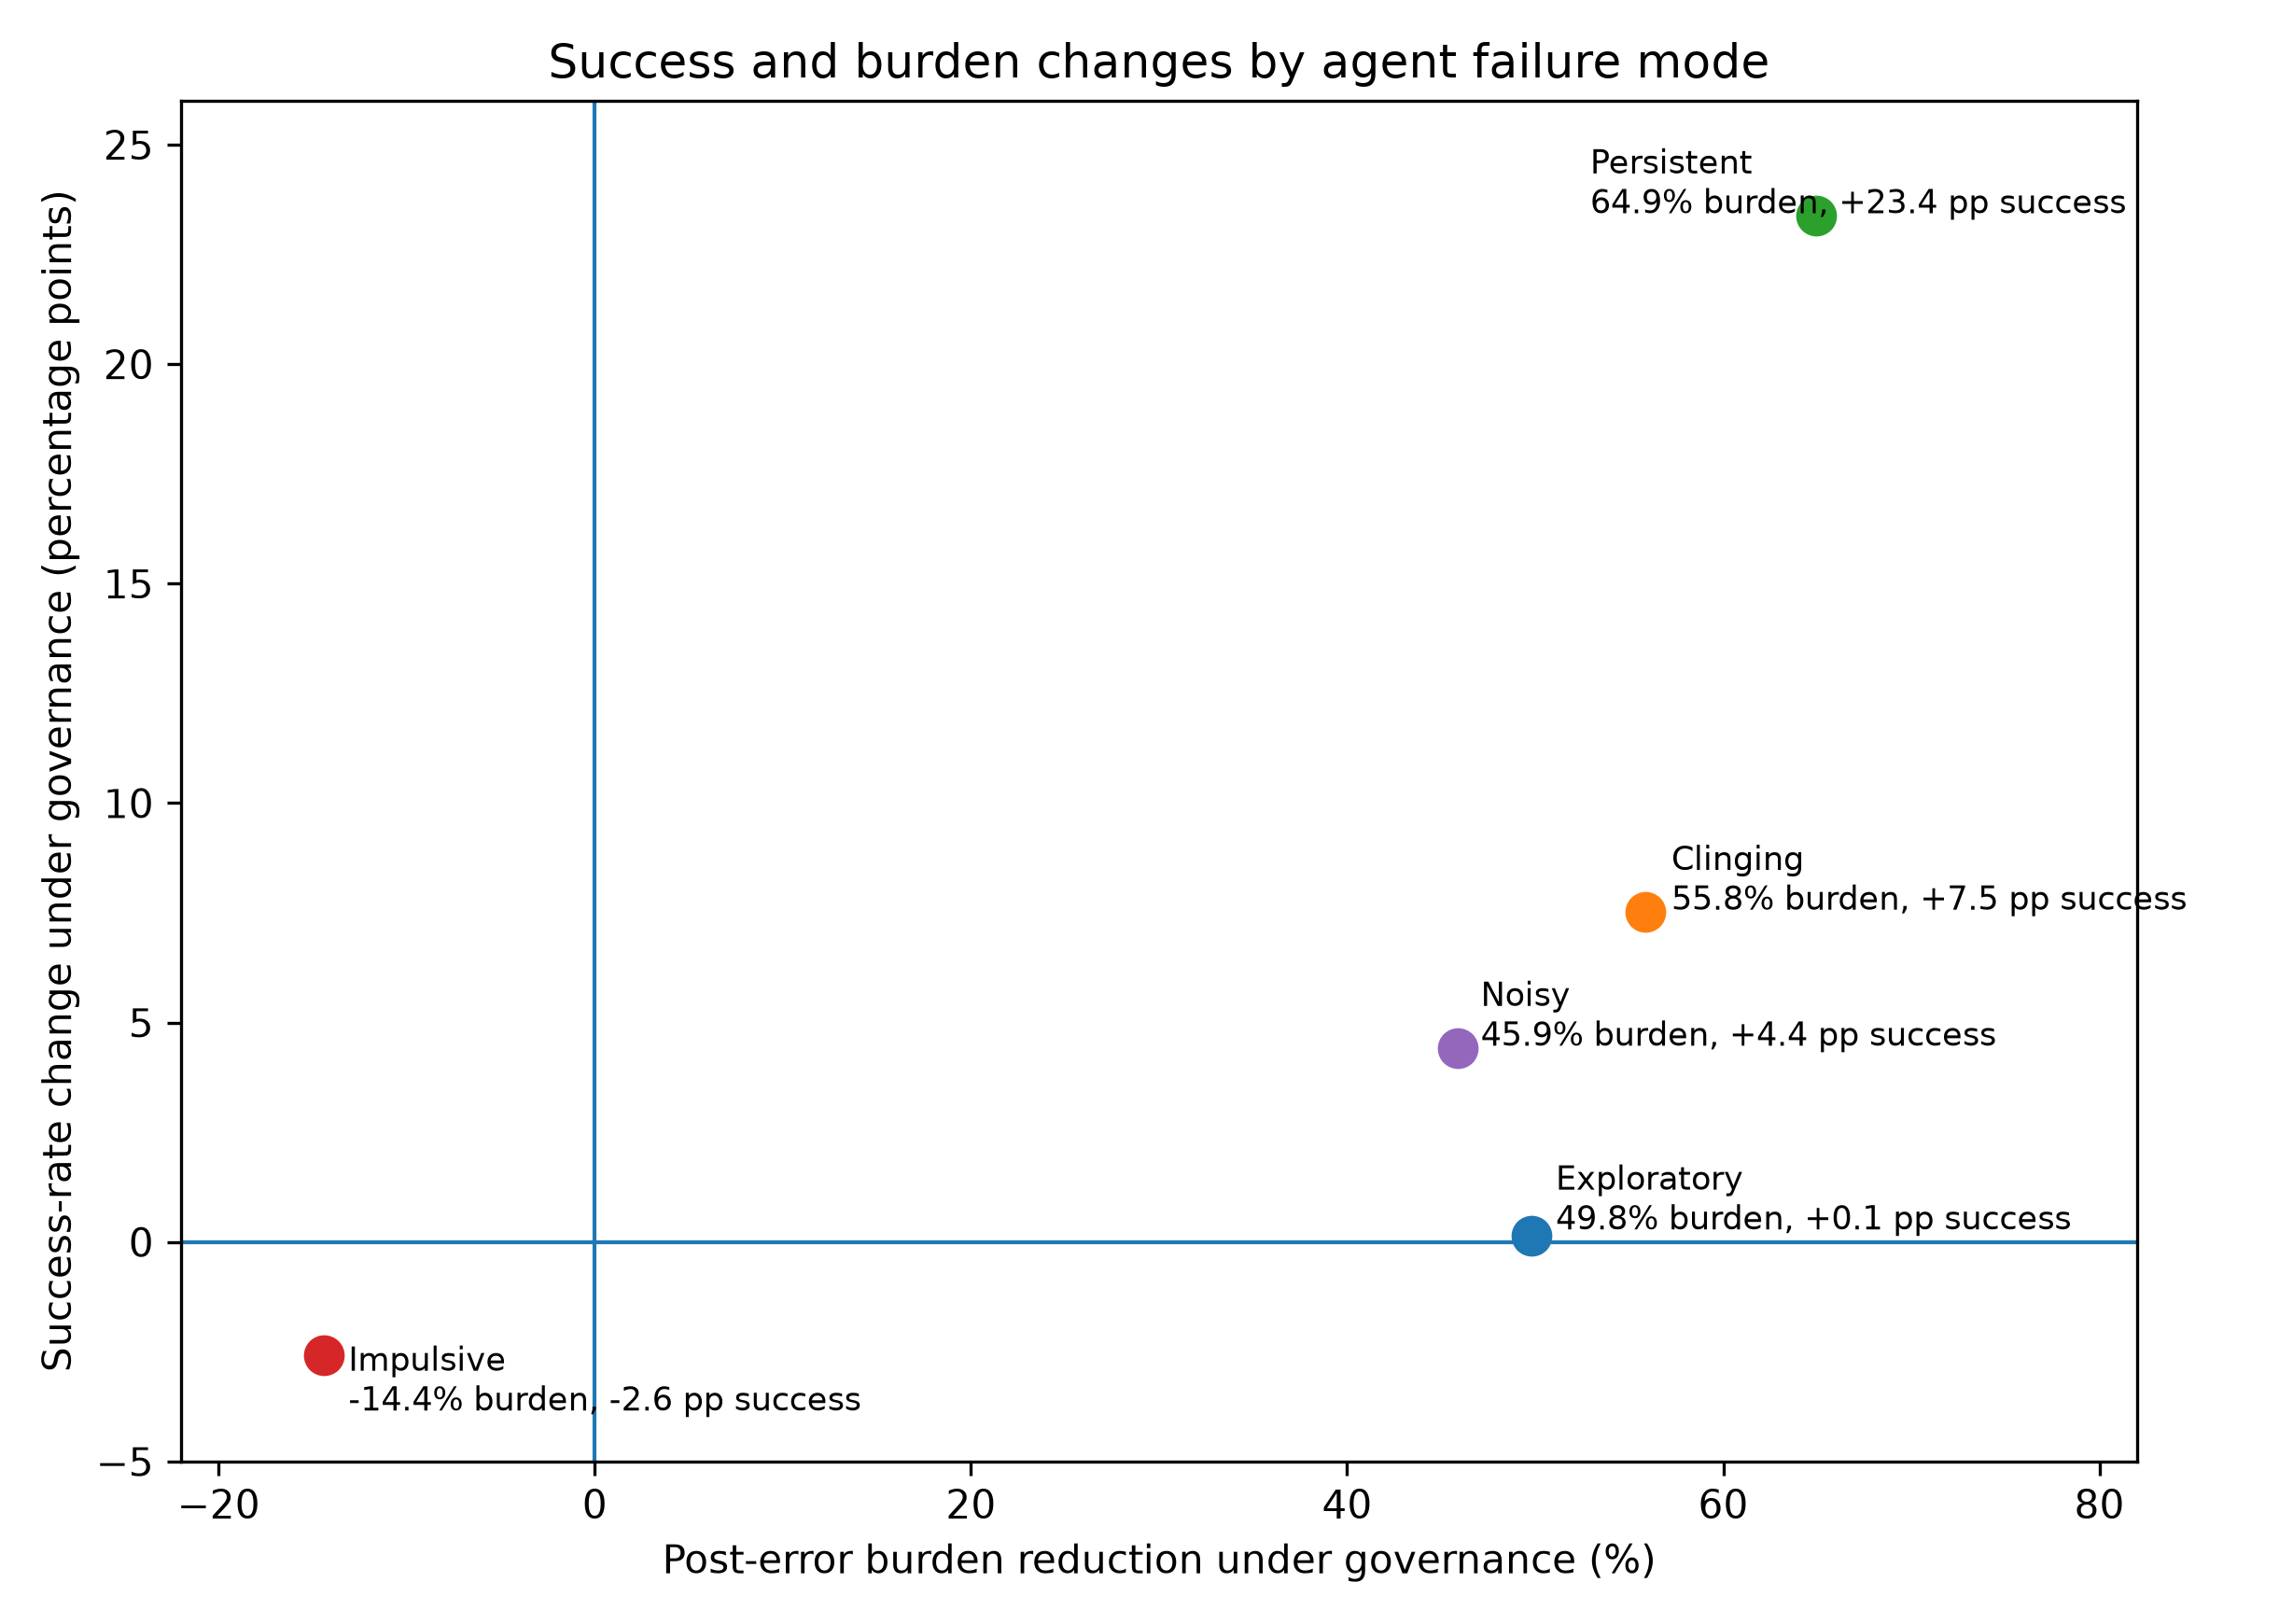
\includegraphics[width=0.92\linewidth]{figures/success_vs_post_error_burden_tradeoff.png}
\caption{Success-burden effects by agent failure mode. Positive horizontal values indicate reduced post-error burden under CAS regulation. Positive vertical values indicate improved success rate. The plot shows that CAS regulation is most beneficial for persistent, clinging, and noisy agents, while the impulsive agent marks a boundary condition.}
\label{fig:tradeoff}
\end{figure}

\section{Discussion}

\subsection{Regulation helps when the failure mode is perseveration}

The main result is that CAS regulation helps most when the agent's failure mode is perseveration after disturbance. Persistent and clinging agents repeatedly attempt failed or unsupported actions in the ungoverned condition. The governor reduces this behavior by changing the control regime after failure. It does not need to know the correct path. It only needs to recognize that the current action pattern has become unproductive.

The noisy agent also benefits because noisy guesses create unnecessary post-error burden. Regulation reduces the impact of this failure mode by favoring more structured uncertainty reduction. The exploratory agent shows a smaller but still positive burden reduction because its baseline policy is already relatively adaptive.

\subsection{Not a general agent-intelligence claim}

These results should not be interpreted as a claim that CAS regulation makes agents generally intelligent. The experiment is narrow. The environment is a controlled file-recovery domain, and the agents are stochastic policies rather than broad reasoning systems. The contribution is more specific: regulatory state modulation can reduce a measurable recovery burden in agents whose post-error policy tends to repeat or drift.

This distinction is important. A governor that reduces repeated failed actions is not the same as a planner that knows the solution. The governor changes how the agent responds to disturbance. It does not replace perception, reasoning, memory, or task knowledge.

\subsection{Not an LLM benchmark}

This study is also not an LLM benchmark. Commercial LLM APIs are difficult to use for this kind of controlled statistical experiment because repeated runs are expensive, rate-limited, and difficult to reproduce. The stochastic model is intentionally used instead. It allows 800,000 controlled runs with known policy classes and repeatable random seeds.

The results can inform future LLM-agent evaluations, but they should not be presented as evidence that a particular language model is improved. A live LLM integration would require a separate study with adequate repetitions, stable API conditions, and clear separation between generic regulation and task-specific prompting.

\subsection{Path toward live tool-using agents}

The next step is to connect this regulatory mechanism to live tool-using agents without turning the regulator into a prompt-based solution script. A fair live-agent study should keep the task, tools, and history identical across conditions, and add only a generic regulatory signal in the governed condition. It should also use enough repetitions to estimate uncertainty. Until those conditions are practical, the stochastic experiment provides the cleaner evidence.

A second path is to replace the hand-coded stochastic policy with a learned policy while keeping the governor separate. For example, a small neural policy could estimate next-action probabilities from trace features, and CAS regulation could modulate the resulting logits or action-class weights. That would test whether the same regulatory principle survives a less hand-specified action-selection mechanism.

\section{Conclusion}

This paper studied post-error burden in stochastic tool-using agents. The CAS Agent Governor reduced repeated failed actions and post-error tool burden by modulating action-selection probabilities according to regulatory state. In an 800,000-run experiment, governance improved success and reduced burden for clinging, persistent, and noisy agents, with the strongest effect for persistent agents. Repeated failed actions were suppressed to zero across all governed agent types.

The result is deliberately narrow. CAS regulation is not a general agent-intelligence mechanism and not an LLM benchmark. It is a control layer for post-error behavior. Its benefit depends on the agent's failure mode. When the failure mode is perseverative or noisy recovery, regulatory modulation can substantially reduce recovery burden. When the baseline agent is already fast and impulsive, the same regulation can add cost. This boundary condition strengthens the interpretation: regulation is useful not because it solves the task, but because it changes how an agent responds when its current strategy has failed.

\section*{Data and code availability}

The experiment is implemented in the CAS Agent Governor codebase. The publication configuration uses \texttt{MAX\_STEPS = 16} and \texttt{SEEDS\_PER\_CONDITION = 10000}. The generated output files include \texttt{stochastic\_policy\_runs.csv}, \texttt{stochastic\_policy\_aggregate.csv}, and the plotted figures used in this paper.

\begin{thebibliography}{9}

\bibitem{ziegler_iram}
V. Ziegler.
\newblock \emph{IRAM-$\Omega$-Q: A Computational Architecture for Uncertainty Regulation in Artificial Agents}.
\newblock Critical Attention Systems, 2026.

\bibitem{ziegler_memory}
V. Ziegler.
\newblock \emph{When Regulation Has Memory: Hysteresis and Control Burden in an Adaptive Artificial Agent}.
\newblock Critical Attention Systems, 2026.

\bibitem{ziegler_intermit}
V. Ziegler.
\newblock \emph{Intermittent Control Is Not Diluted Control: A Switching Effect in Artificial Agency}.
\newblock Critical Attention Systems, 2026.

\bibitem{ziegler_burden}
V. Ziegler.
\newblock \emph{Control Burden and Regulatory Demand in Adaptive Artificial Agents}.
\newblock Critical Attention Systems, 2026.

\end{thebibliography}

\end{document}
